Tratta dell'ottimizzazione degli Algoritmi e della scelta del piano fisico:\\
\textbf{Algoritmi}
\begin{itemize}
    \item per l’elaborazione dei singoli operatori logici
    \item per l’elaborazione complessiva del piano fisico
\end{itemize}
\textbf{Scelta del piano fisico}
\begin{itemize}
    \item stima della dimensione dei risultati e del costo di un piano di esecuzione
    \item identificazione dello spazio di ricerca dei piani
    \item trattamento delle sottointerrogazioni
\end{itemize}

\subsection{Pieni di esecuzioni fisici}
Ogni piano di esecuzione fisico si compone di una serie di operatori fisici connessi ad albero. Le sue foglie sono le relazioni di base presenti nel piano logico ottimizzato. Gli altri nodi sono operatori che agiscono su 1 o 2 insiemi di tuple in input e producono 1 insieme di tuple in output.

\subsection{Operatori fisici}
Sono implementazioni specifiche di un operatore logico (ad esempio del join).\\
Vengono scelti in funzione dei valori delle statistiche, dei parametri di sistema (es. dimensione del buffer pool) e della logica dell'algoritmo.\\
Per ogni operatore logico, esistono diversi algoritmi di realizzazione.\\
Tecniche alla base degli operatori fisici:
\begin{itemize}
    \item \textbf{iterazione}: si esaminano le tuple della relazione di input sequenzialmente (scansione sequenziale)
    \item \textbf{indici}: se è specificata una selezione o una condizione di join su una relazione di base, si usa un indice per esaminare solo le tuple che soddisfano la condizione.
    \item \textbf{partizionamento}: si partizionano le tuple in base ad una chiave (ad esempio usando una funzione hash) si decompone il problema eseguendo l’operazione prima sulle partizioni (più piccolo, meno costoso) e poi si integrano i risultati.
\end{itemize}
Il costo tiene conto delle operazioni di I/O escludendo le operazioni di Output siccome non \`e detto che il risultato debba essere scritto su disco.

\break
\subsection{Cammini di accesso}
Le foglie dei piani di esecuzione sono sempre tabelle di base. Un cammino di accesso descrive come accedere al file dei dati di una relazione per ritrovare le tuple di interesse e tiene conto di eventuali operazioni di selezione definite sulle relazioni di base, per le quali esista un indice utilizzabile per la loro esecuzione.
\begin{itemize}
    \item \textbf{Scansione Sequenziale}
    \item \textbf{Indice più una condizione di ricerca}
\end{itemize}
Un indice può essere utilizzato come cammino di accesso a una relazione solo se esiste una condizione di selezione che può essere eseguita utilizzando l’indice.\vspace{2mm} \\
In presenza di \textbf{condizioni composte} il sistema preferisce scegliere un PQP (Physical Query Processor) che contenga un cammino di accesso basato su una condizione con indice che, se falsa, rende falsa tutta l’interrogazione (\textbf{fattore booleano}).\\
Esempio di Fattore booleano:\\
\indent La seconda condizione dell'\code{AND} in: \code{(R.A = 5 OR R.B = 6) AND R.C > 10}\vspace{2mm} \\
Può anche essere scelto più di un cammino di accesso, combinando poi i risultati con un ulteriore operatore fisico: \code{A=5 AND B=6} => 2 index scan con \code{INTERSECTION} fra i risultati

\subsection{Costi}
\begin{itemize}
    \item \textbf{Scansione sequenziale}: Numero dei blocchi. Unica opzione in assenza di indici, devo vedere tutta la tabella.
    \item \textbf{Accesso con indice}: 1 in caso di indice hash, $h (\log N)$ per indice ad albero, $+$ costo per accedere ai blocchi dei dati. (Clusterizzazione influisce sul costo di quest'ultimo)
\end{itemize}

\subsection{Rimozione dei duplicati (DISTINCT)}
Tre possibili approcci (ne vediamo solo due):
\begin{itemize}
    \item Ordinamento
    \item Indici
    \item \sout{Hashing}
\end{itemize}

\subsubsection{Ordinamento}
\begin{enumerate}
    \item Si accede sequenzialmente a R per ottenere un insieme di tuple che contengono solo gli attributi desiderati
    
    \item Si ordina questo insieme di tuple rispetto a tutti gli attributi di proiezione (vedremo in seguito come si implementa l’ordinamento)
    
    \item Si scandisce il risultato ordinato, eliminando le tuple duplicate (che sono adiacenti)
\end{enumerate}

\subsubsection{Indici}
Per proiezioni su relazioni di base, se esiste un indice ordinato (denso) con chiave di ricerca uguale alla lista di proiezione, si può accedere a tutte le foglie dell'indice invece che al file dei dati.

\subsection{Ordinamento}
Ci sono due approcci:
\begin{itemize}
    \item Merge sort a due fasi
    \item $\text{B}^+$ tree
\end{itemize}

\subsubsection{Merge sort a due fasi}
\begin{enumerate}
    \item Vengono portate nel buffer il più possibile numero di pagine, vengono ordinate internamente e i risultati salvati in un file temporaneo.
    \item Merge delle pagine ordinate nella fase 1
\end{enumerate}

\subsubsection{\texorpdfstring{$\text{B}^+$}{TEXT} tree}
Ottimo quando l'indice \`e clusterizzato. Si usano le foglie dell'albero per ordinare.
\begin{enumerate}
    \item si trovano le foglie dell’indice che soddisfano la condizione
    \item si ordinano i rid dei record dei dati da reperire, in modo che i rid di record nello stesso blocco siano vicini
    \item si accede ai record corrispondenti in ordine
\end{enumerate}

\subsection{Join}
Tipi di join:
\begin{itemize}
    \item Nested Loop Join
    \item Index Nested Join
    \item Merge Join
    \item Hash Join
\end{itemize}
$$R \bowtie S$$
$$\text{Outer} \bowtie \text{Inner}$$

\subsubsection{Iterazione semplice (Nested Loop Join)}
$B() =$ Blocchi\\
$T() =$ Tuple\\
Costo: $B(R) + T(R) * B(S)$\\
Siccome la relazione inner viene scandita per ogni tupla di quella outer e quindi "scorre più velocemente" \`e conveniente usare la relazione più piccola come inner, specialmente se può essere contenuta in main memory.

\subsubsection{Block Nested Loop}
Usata come variante dell'Iterazione semplice. Esegue il Join blocco per blocco invece che tupla per tupla.

\subsubsection{Index Nested Loop}
Scandisce gli indici invece dell'intera tabella.\\
Costo: $T(R) + T(R) * \text{Costo ricerca nell'indice di S}$

\subsubsection{Merge Join}
Il Merge Join sfrutta l'ordinamento di entrambi gli insiemi di tuple in input.\\
Usabile se:
\begin{itemize}
    \item Relazioni Clusterizzate su un indice ordinato
    \item Relazioni NON Clusterizzate ma con indice ordinato
\end{itemize}
Sfrutta l'ordinamento per non eseguire confronti inutili.\\
\textbf{Generalmente usato con join di uguaglianza}.

\subsubsection{Hash Join}
L’algoritmo di Hash Join, applicabile solo in caso di equi-join, non richiede né la presenza di indici né input ordinati.\\
Usa funzioni di Hash per confrontare i valori uguali.

\subsection{Elaborazione del piano fisico}
\subsubsection{Materializzazione}
Ogni volta che si esegue un operatore, il risultato viene scritto in memoria come tabella temporanea partendo dagli operatori più in basso nell'albero.

\subsubsection{Pipeline}
Si eseguono gli operatori uno dopo l'altro per ogni tupla invece di aspettare il completamento passando l'output di un operatore come input al prossimo. Non \`e sempre possibile.\\
Casi in cui \`e utilizzabile:
\begin{itemize}
    \item Proiezione con dupplicati
    \item Selezione con algoritmo di iterazione
    \item Join con algoritmi di iterazione (Nested Loop)
    \item Join con uso di indici
\end{itemize}

\subsection{Stima del Costo}
Si stima il costo per ogni nodo dell'albero stimando anche la dimensione del suo risultato e se \`e ordinato o meno. Alla fine si sommano i costi parziali ottenuti.\\
Per effettuare le stime si usano delle \textbf{statistiche} contenute nei cataloghi di sistema.\\
Le statistiche contengono:\\
\textbf{Per ogni relazione $R$}:
\begin{itemize}
    \item $T(R)$: Tuple
    \item $B(R)$: Blocchi
    \item $S(R)$: Dimensione (media se lunghezza variabile) di ogni tupla
    \item $S(A, R)$: Dimensione dell'attributo $A$
    \item $V(A, R)$: Valori Distinti dell'attributo $A$
    \item $Max(A, R), Min(A, R)$: Valore minimo o massimo dell'attributo $A$ in $R$
\end{itemize}
\textbf{Per ogni indice $I$}:
\begin{itemize}
    \item $K(I)$: Entrate
    \item $L(I)$: Pagine foglia
    \item $H(I)$: Altezza
\end{itemize}
Le statistiche vengono aggiornate alla creazione di un indice o periodicamente (non ad ogni modifica). Esempio comando \code{ANALYZE}

\subsection{Stima della dimensione della selezione}
\textbf{Fattore di selettività} $F(P)$ = $\text{Numero di tuple che soddisfano la selezione}/\text{tuple totali}$\\
Si stima assumendo una \textbf{distribuzione uniforme} dei valori di ogni attributo.
\begin{itemize}
    \item $F(A=v) = \frac{1}{V(A, R)}$
    \item $F(A \text{ IN } (v_1, v_2, ..., v_N)) = N * F(A = v)$
    \item $F(A > v) = \frac{Max(A, R) - v}{Max(A, R) - Min(A, R)}$
    \item $F(A < v) = \frac{v - Min(A, R)}{Max(A, R) - Min(A, R)}$
    \item $F(A = B) = \frac{1}{Max(V(A, R), V(B, R))}$
    \item $F(C_1 \text{ AND } C_2) = F(C_1) * F(C_2)$
    \item $F(C_1 \text{ OR } C_2) = F(C_1) + F(C_2) - F(C_1) * F(C_2)$
    \item $F(\text{NOT }C) = 1 - F(C)$
\end{itemize}

\break
\subsection{Ottimizzazione Join Multipli}
Si considerano solo \textbf{piani left-deep}, cioè che generano un albero dove ogni \code{JOIN} ha come operatore esterno il risultato degli altri \code{JOIN}
\begin{figure}[htbp]
    \centering
    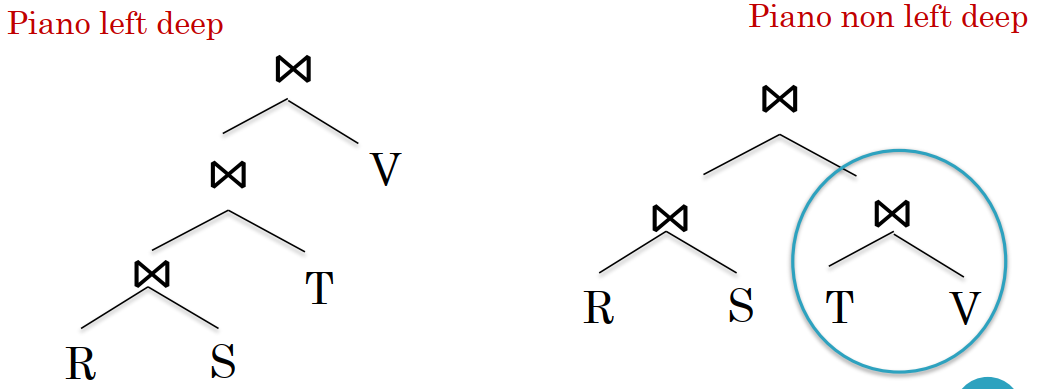
\includegraphics[width=0.9\textwidth, keepaspectratio]{leftdeep.png}
    \label{fig:leftdeep}
\end{figure}

\subsection{Sottointerrogazioni}
\begin{itemize}
    \item Se \`e possibile, vengono rimosse
    \item Se sono scalari, viene calcolato il risultato una volta
    \item Se sono correlate devono invece essere eseguite ogni volta
\end{itemize}